\mySection{10.5 Contingency Tables}
%-------------- start slide -------------------------------%{{{ 10.44
\begin{frame}[2-]
	% {\S\: 10.5 Contingency Tables}
	\begin{enumerate}
		\item[E.g. 1] Whether are the two ratings independent?
			\vfill
			\begin{center}
				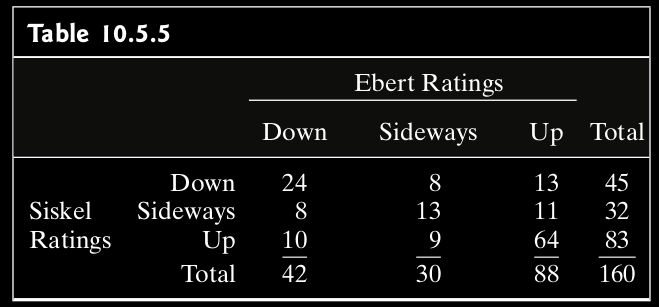
\includegraphics[scale=0.3]{Table_10-5-5-neg.png}
			\end{center}
	\end{enumerate}
\end{frame}
%-------------- end slide -------------------------------%}}}
%-------------- start slide -------------------------------%{{{ 10.45
\begin{frame}[2,4]
	\begin{enumerate}
		\item[E.g. 2] Whether is the suicide rate independent of the mobility factor?
			\vfill
			\begin{center}
				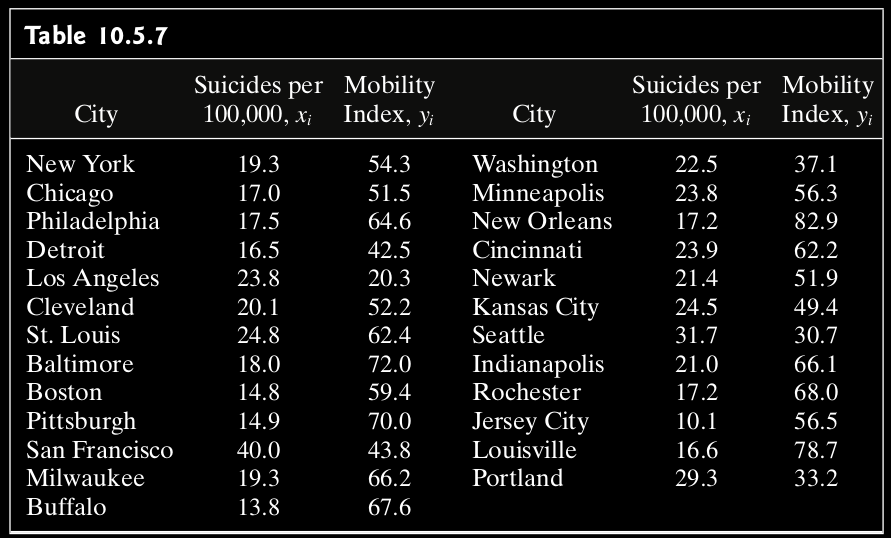
\includegraphics[scale=0.25]{Table_10-5-7-neg.png}
			\end{center}
			\pause
		\item[]\[
				\bar{x} = 20.8\quad\text{and}\quad \bar{y} = 56.0
			\]
			\begin{center}
				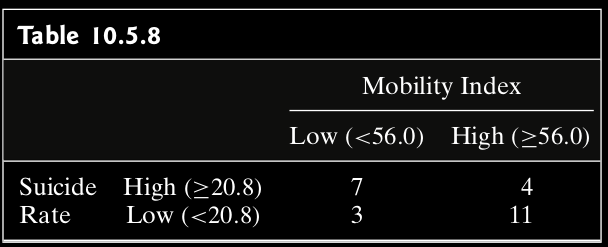
\includegraphics[scale=0.25]{Table_10-5-8-neg.png}
			\end{center}
	\end{enumerate}
\end{frame}
%-------------- end slide -------------------------------%}}}
%-------------- start slide -------------------------------%{{{ 10.46
\begin{frame}
	\begin{enumerate}
		\item[Thm \small 10.4.1] Suppose that $n$ observations are taken on a sample space partitioned by the
			events $A_1,\cdots, A_r$ and $B_1,\cdots,B_c$. \\[1em]
		\item[] Let $p_i=\bbP(A_i)$, $q_j = \bbP(B_j)$, $p_{ij} = \bbP(A_i\cap B_j)$.\\[1em]
		\item[] Let $X_{ij}$ be the number of observations belonging to $A_i\cap B_j$.
			\vfill
		\item[a)] Provided that $np_{ij}\ge 5$ for all $i,j$, the r.v.
			\[
				D_2 = \sum_{i=1}^r \sum_{j=1}^c  \frac{\left(X_{ij}-np_{ij} \right)^2}{np_{ij}} \sim \text{Chi square of f.d. $rc-1$}
			\]
			\vfill
		\item[b)] To test $H_0:$ $A_i$'s are independent of $B_i$'s, calculate the test statistic
			\[
				d_2 = \sum_{i=1}^r \sum_{j=1}^c  \frac{\left(k_{ij}-n\hat p_{i}\hat q_j \right)^2}{n\hat p_{i}\hat q_j}
			\]
			where $\hat p_i$ and $\hat q_j$ are MLE's for $p_i$ and $q_j$, respectively.\\[1em]
		\item[] Provided that $n\hat p_i \hat q_j\ge 5$ for all $i,j$, the critical region is
			\[
				(\chi^2_{1-\alpha,(r-1)(c-1)},+\infty)
			\]
	\end{enumerate}
\end{frame}
%-------------- end slide -------------------------------%}}}
%-------------- start slide -------------------------------%{{{ 10.47
\begin{frame}[2-]

	\begin{enumerate}
		\item[E.g. 1] Sol: Compute the expected frequencies:\\[1em]
			\begin{center}
				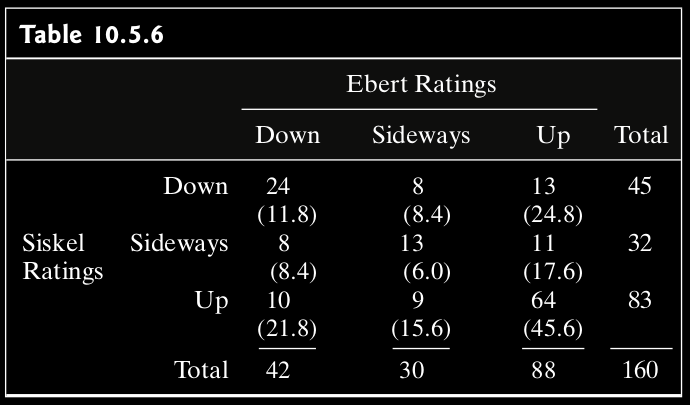
\includegraphics[scale=0.25]{Table_10-5-6-neg.png}
			\end{center}
			\pause
		\item[]
			\[
			\Longrightarrow \quad d_2 = \cdots = 45.37
			\]
			\vfill
		\item[] Critical region is
			\[
				\left(\chi^2_{0.99,(3-1)\times (3-1)},+\infty \right) = (13.277,+\infty)
			\]
		\item[] Alternatively $P$-value = $\bbP(\chi^2_4 \ge 45.37)=   3.33\times 10^{-9}$.
			\vfill
		\item[] Rejection at $\alpha=0.01$.\myEnd
	\end{enumerate}
\end{frame}
%-------------- end slide -------------------------------%}}}
%-------------- start slide -------------------------------%{{{ 10.48
\begin{frame}[2-]

	\begin{enumerate}
		\item[E.g. 2] Sol: Compute the expected frequencies:\\[1em]
			\begin{center}
				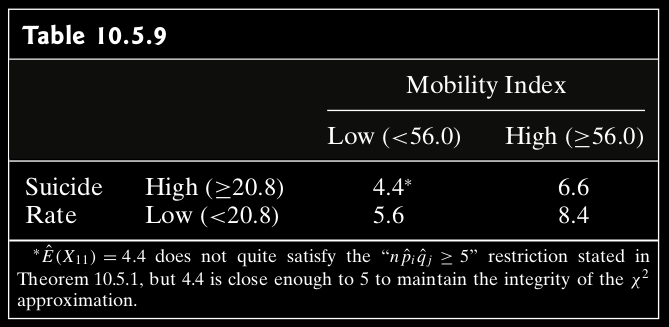
\includegraphics[scale=0.25]{Table_10-5-9-neg.png}
			\end{center}
			\pause
		\item[]
			\[
			\Longrightarrow \quad d_2 = \cdots = 4.57
			\]
			\vfill
		\item[] Critical region is
			\[
				\left(\chi^2_{0.95,(2-1)\times (2-1)},+\infty \right) = (3.41,+\infty)
			\]
		\item[] Alternatively $P$-value = $\bbP(\chi^2_1\ge 4.57)=  0.033$
			\vfill
		\item[] Rejection at $\alpha=0.05$.\myEnd
	\end{enumerate}
\end{frame}
%-------------- end slide -------------------------------%}}}
